
\section {Servidor de alarmes BEAST}
%\subsection{Introdução}

\begin{frame}
\frametitle{Servidor de alarmes BEAST}
\framesubtitle{Introdução}
\begin{itemize}
  \item Mantido pelo SNS (\textit{Oak Ridge National Laboratory}).
  \item Implementado em \textit{Java} e baseado no \textit{Eclipse}.
\end{itemize}

\begin{figure}[h]

\centering
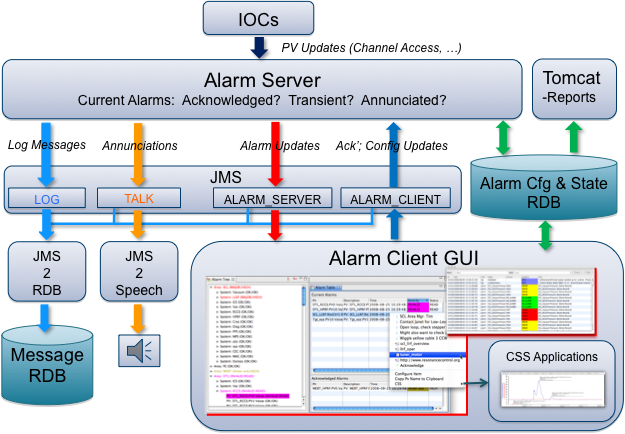
\includegraphics[width=0.6\textwidth]{image/beast-arquitetura}
\caption {Implementação do sistema de monitoramento de alarmes
\textit{BEAST}.}
\label{fig:best_arquitetura}
\end{figure}

\end{frame}

%\subsection{Instalação}

\begin{frame}
\frametitle{Servidor de alarmes BEAST}
\framesubtitle{Cliente do Servidor de Alarmes - CSStudio}
\begin{figure}[h]
\centering
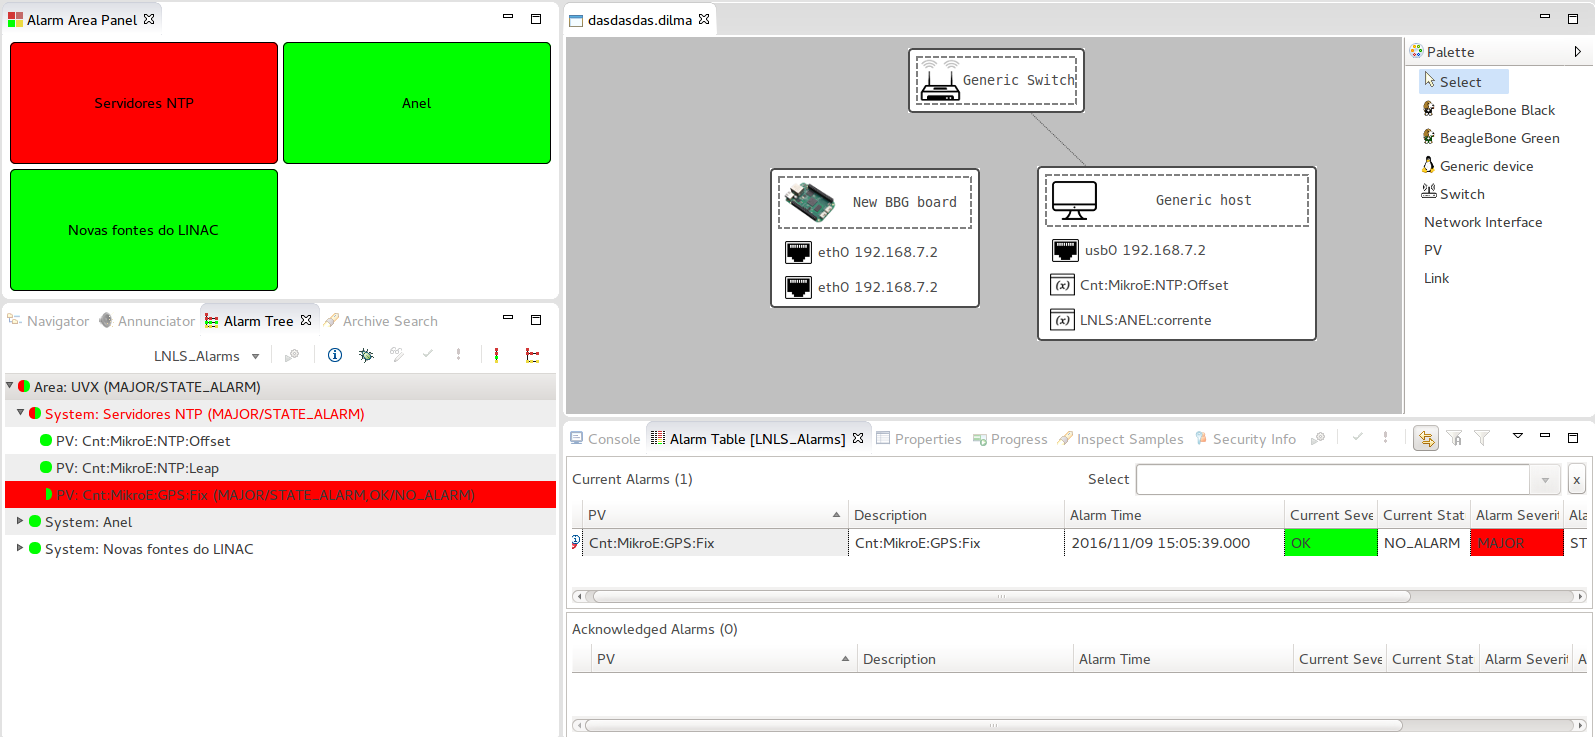
\includegraphics[width=\textwidth]{image/beast-screen-shot}
\caption {Cliente \textit{BEAST} baseado no \textit{Control System Studio}.}
\label{fig:alarm}
\end{figure}

\end{frame}

\begin{frame}
\frametitle{Servidor de alarmes BEAST}
\framesubtitle{Plugin \textit{Monitor} desenvolvido}
\begin{figure}[h]
\centering
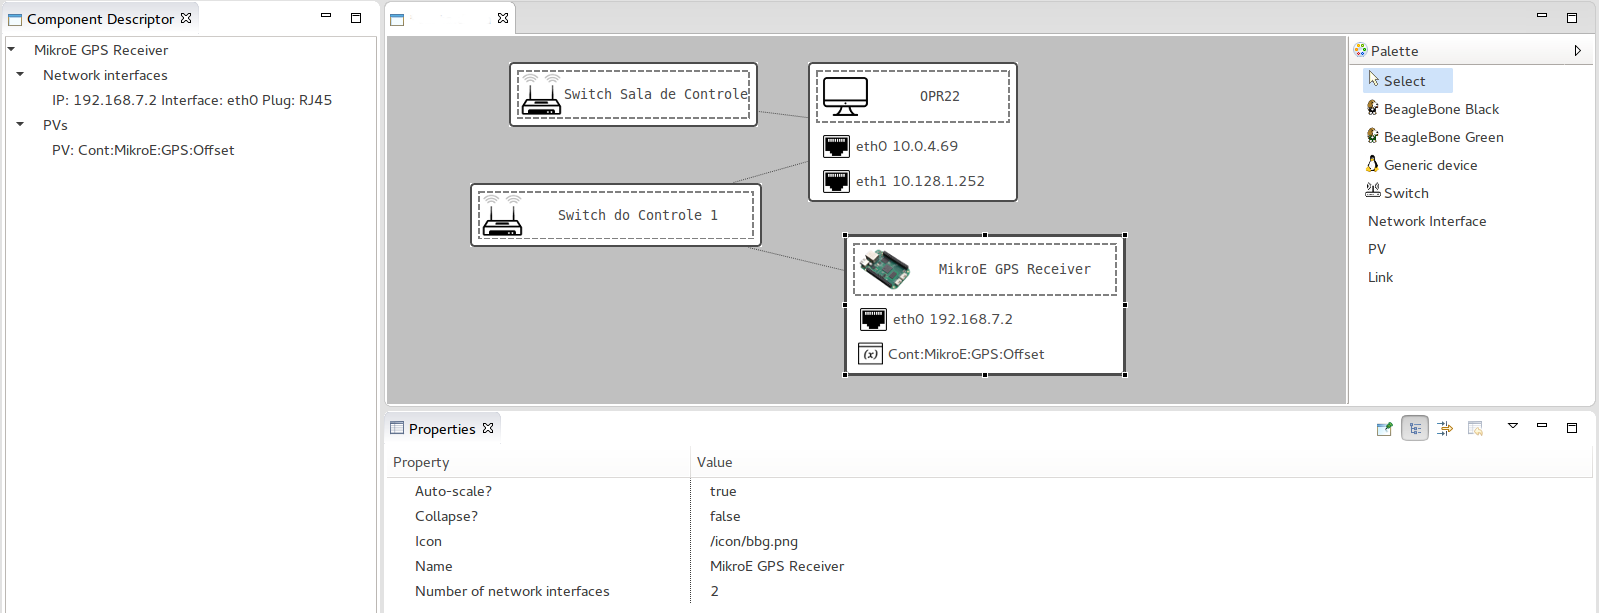
\includegraphics[width=\textwidth]{image/plugin}
\caption {\textit{Plugin} desenvolvido com base no GEF3.}
\label{fig:plugin}
\end{figure}

\end{frame}


%\subsection{Obtendo o LNLStudio}

\begin{frame}
\frametitle{Servidor de alarmes BEAST}
\framesubtitle{LNLStudio - CSStudio 4.3.4 e Mars}
\begin{figure}[h]
\centering
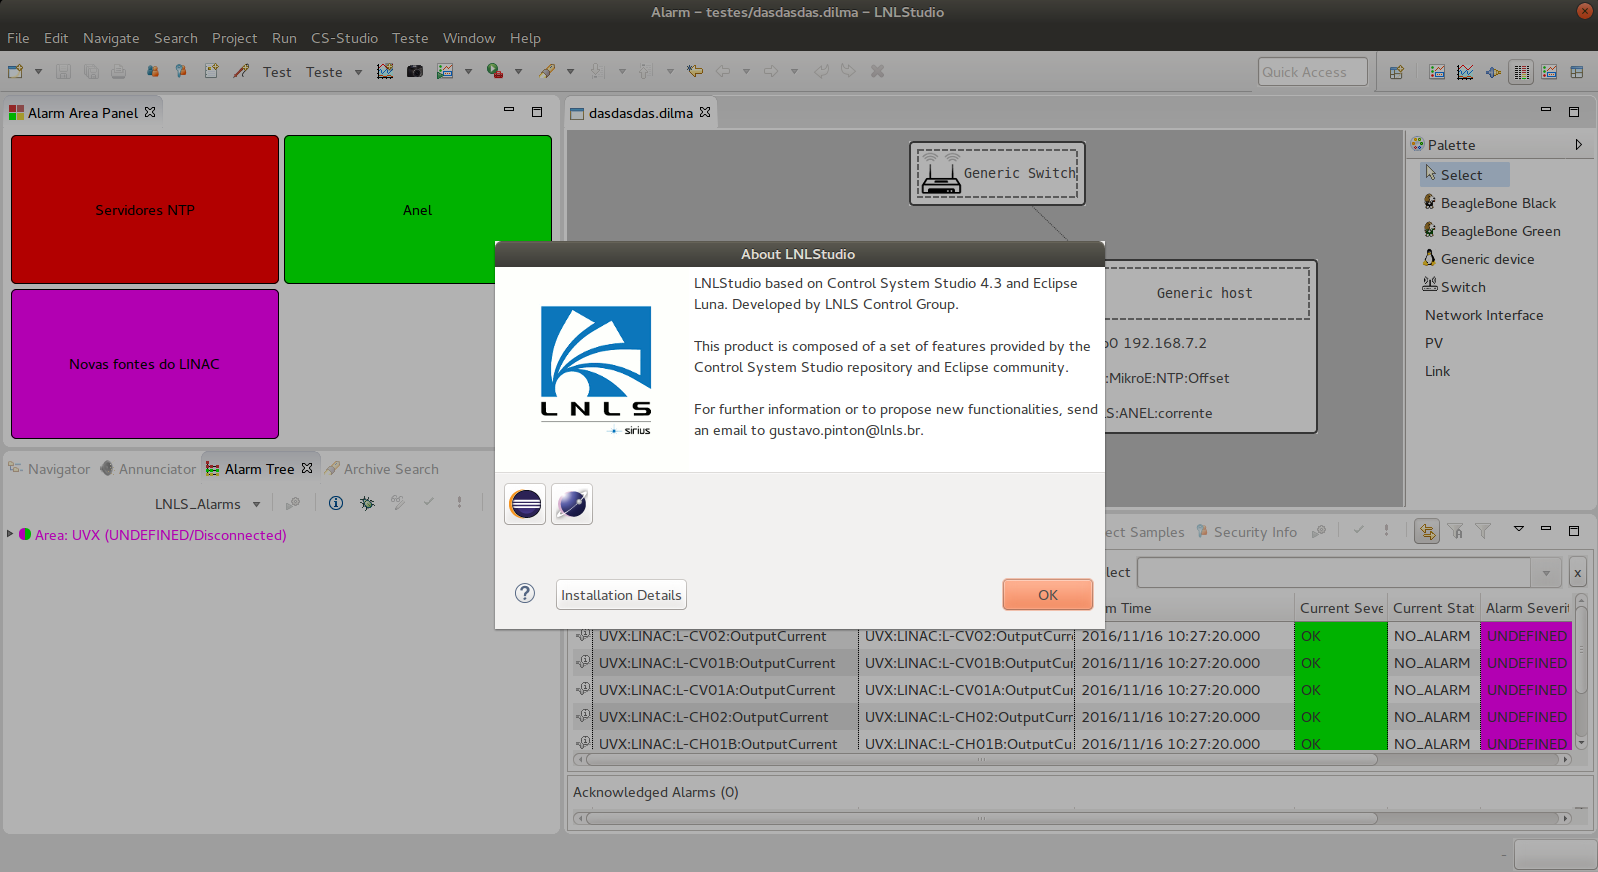
\includegraphics[width=0.90\textwidth]{image/lnlstudio}
\caption {\centering Produto \textit{LNLStudio} exportado a partir de uma
configuração do \textit{Eclipse}.}
\label{fig:lnlstudio}
\end{figure}

\end{frame}
